\documentclass[main.tex]{subfiles}
\graphicspath{{./img}}

\begin{document}
\section{System validation} \label{sec-validation}

This section will be devoted to the evaluation and demonstration of the proposed MAS-based ITS
implementation framework. An ITS solution will be chosen to demonstrate implementation using 
the framework, serving as a validation of the system design. The chosen ITS solution will be simulated
in the IVS software by using the proposed framework. The implementation process will be documented, 
and the simulation results will be discussed.

\subsection{Qualitative analysis}

The following paragraphs will pick up on the findings in the chapter (\ref{sec-croads}), where the
table (\ref{gdt-mapping}) maps General Driving Tasks to state-of-the-art ITS solutions. Those
ITS solutions will be analyzed in this chapter in an attempt to transparently select an optimal
system to implement using the developed framework in order to validate and demonstrate its
use-case. 

In order to choose an optimal ITS to implement, it is important to define features that 
reflect such system's suitability for implementation. Optimally selecting such features 
for evaluation of previously selected individual ITSs will create a qualitative benchmark that
will be used to select an ITS solution for demonstration of the proposed framework's
capabilities.

The method to determine how well-suited the candidate system type is for the implementation to
an IVS will be to evaluate it based on the \emph{three} features discussed in the preceding
section (\ref{sec-its}): 

\begin{itemize}
    \itemspacing{.5}
    \item Intelligence distribution rate
    \item Driver engagement
    \item Research relevance
\end{itemize}

A set of integer values will determine the rates how the selected features are represented in the 
ITS solution in question. The representation level will be expressed in a fuzzy logic given in four levels:

\begin{itemize}
    \itemspacing{.5}
    \item \talign{None}{5}{$\rightarrow$\quad 0}
    \item \talign{Low}{5}{$\rightarrow$\quad 2}
    \item \talign{Moderate}{5}{$\rightarrow$\quad 5}
    \item \talign{High}{5}{$\rightarrow$\quad 8}
\end{itemize}

Because \emph{None} representation of the feature does not bear any significance to choosing an ITS 
in question, it will be assigned zero. \emph{Low} representation should not have a significant impact on 
the suitability of ITS, therefore its value is only incremented by two as opposed to \emph{None}. \emph{Moderate}
and \emph{High} rates of feature representation should have a more significant influence on the final system 
choice, therefore their values have been assigned as increments of three instead of two. 

Each system reviewed in section (\ref{sec-its}) will be evaluated and the sum of individual feature evaluation 
will determine its score, meaning the higher the score, the better the result for a particular ITS. The system 
with the \emph{highest} score will be chosen to implement using the proposed framework. The results of the 
qualitative analysis can be seen in the table (\ref{qa-table}) below.

\begin{table}[htbp]
    \caption{Quantitative analysis results}
    \renewcommand{\arraystretch}{1.4}
    \centering\begin{tabular}{l*{3}{r}r} \toprule
         & \multicolumn{3}{c}{Features} & \\ \cmidrule(rl){2-4}
        ITS & \multicolumn{1}{p{6em}}{MAS-compatibility} & \multicolumn{1}{p{6em}}{Driver \newline engagement} & \multicolumn{1}{p{6em}}{Research \newline relevance} & \textbf{Score } \\ \midrule
        E-Call & 2 & 2 & 5 & 9 \\ 
        Electronic fee collection & 2 & 0 & 2 & 4 \\
        Parking guidance & 2 & 8 & 5 & 15 \\
        Network traffic control & 8 & 0 & 8 & 16 \\
        \textbf{Cooperative ACC} & 8 & 8 & 8 & \textbf{24} \\
        European Truck Platooning & 5 & 2 & 8 & 15 \\
        ADASIS & 2 & 8 & 8 & 18 \\
        Mobility as a Service & 8 & 2 & 8 & 18 \\
        Map services (Geo-fencing) & 2 & 5 & 8 & 15 \\
        \multicolumn{1}{p{5em}}{Self-driving algorithms} \& Platooning & 8 & 2 & 8 & 18 \\
        \textbf{IVIS} & 8 & 8 & 8 & \textbf{24} \\ \bottomrule
    \end{tabular}
    \label{qa-table}
\end{table}

\subsubsection{Results discussion}

The conducted analysis has determined two ITS solutions as suitable systems to demonstrate 
implementation - IVIS-based awareness and warning information system and Green
Light Optimal Speed Advisory. Both these come from the state-of-the-art C-ITS subfield. As 
previously discussed, the GLOSA system is using dedicated message types in its implementation -
the SPaT and MAP messages. On the other hand, the IVIS system can use the pre-implemented 
CAM and DENM messages to share traffic-related information. For this reason, the 
\emph{IVIS-based awareness and warning information system} will be chosen to implement 
using the proposed framework.

\subsubsection{Conclusion}

A methodology for qualitative analysis was introduced and used to
determine the best ITS candidates for implementation into an IVS. The resulting best-fitted
systems were both from the C-ITS field, as their features are much alike those of multi-agent
systems. Finally, the chosen systems to implement were the \emph{IVIS-based awareness and
warning information system} and the \emph{Green Light Optimal Speed Advisory} system. The
following practical part will be dedicated to the implementation methodology, introduction to
the development system and the development itself.

\subsection{IVIS implementation}

With the particular ITS implementation decided, the whole process of implementation will be 
described. Before describing the implementation process itself, a description of the 
implemented IVIS solution will be given, together with implementation requirements and expected
results. Afterward, the custom testing environment setup (i.e. the system implementation) will % TODO reword
be presented. Finally, the implementation test results will be presented and discussed.

\subsubsection{System description \& requirements}

As has been described in the chapter (\ref{sec-its}), the In-Vehicle Information System can enable 
the driver to control various aspects of vehicle set-up, as well as provide (relevant) information about 
the vehicle and the environment, including traffic conditions. The state-of-the-art IVIS solutions include 
V2X communication where vehicles and the infrastructure can distribute otherwise locally-available 
information to all interested road users. 

One such V2X communication use-case referred to as \emph{Smart Routing}, is providing traffic
\emph{real-time} traffic condition information to relevant connected vehicles. For instance,
suppose there is congestion forming at a particularly busy road stretch. The local roadside
equipment can automatically collect accurate traffic density data of connected vehicles
broadcasting awareness messages, process the collected information and in turn broadcast
information about local congestion to other remote road users that can optimize their route
planning using received information \cite{Kotsi2020}.

% \begin{figure}[htbp]
%     \centering
%     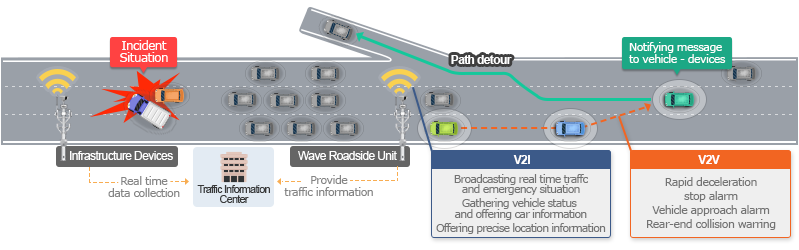
\includegraphics[width=.8\textwidth]{cits-ivis.png}
%     \caption{Illustration of C-ITS use-cases}
%     \label{cits-ivis}
% \end{figure}

In order to successfully build and verify the implementation of the system in the IVS software, 
initial requirements and expected outputs need to be set. The implementation should conform to 
the following specification:

\begin{enumerate}
    \item Intelligent agents should be created using the proposed framework's interface.
    \item The agents should be able to communicate through the standard C-ITS communication protocol.
    \item There should be two types of ITS agents - the connected vehicle agent and the connected infrastructure agent.
    \item The infrastructure agent should be able to detect emerging congestion forming nearby.
    \item Likewise, the agent should also detect that the congestion has decreased.
    \item The congestion event should be specified by the appropriate Cause Code - \texttt{TrafficSituation}.
    \item Similarly, the event status should be specified with a Sub-Cause Code value - 1 for
    free flow and 4 for heavy traffic jam \cite{ETSI2019}. 
    \item The connected vehicle agent should then be able to commit to a plan where it attempts to reach a
    destination, \emph{potentially re-planning its route if it receives a DENM message about a downstream congestion forming}.
 \end{enumerate}

If these conditions are met, the system should have a positive effect on traffic by decreasing the overall 
travel time for vehicles. The implementation will be validated by collecting and analyzing traffic data from 
the simulation.

\subsubsection{External dependencies}

In order to facilitate the validation experiment setup and keep the experiment scope to C-ITS
Smart Routing system implementation, additional packages available to use in the simulation
software will be utilized to model the traffic. Below is a brief overview of the external packages.

\textbf{EasyRoads3D by AndaSoft} \smallskip \\
This package allows one to easily build roads directly in the Unity UI. The main advantage of the 
package is usage simplicity and friendly UI - the user can create road stretches using simple
mouse-based UI with the possibility to connect road segments to create intersections
and build a road network.

With this tool, a testing road network will be built that the vehicle agents will drive through.

\begin{figure}[htbp]
    \centering
    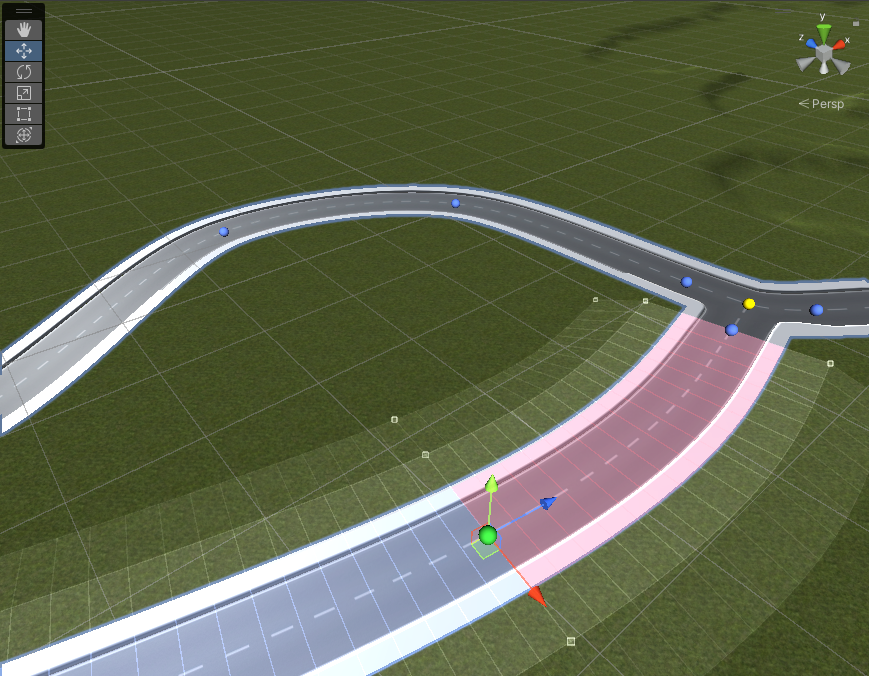
\includegraphics[width=.8\textwidth]{easy-roads.png}
    \caption{EasyRoads3D - The road building UI showcase}
    \label{fig-easyroads}
\end{figure}

\textbf{Simple Traffic System by TurnTheGameOn} \smallskip \\
This package can be used to easily generate vehicle traffic. The traffic is set up by creating
waypoint-based routes that can be interconnected in a modular way to populate road networks
with traffic. Vehicles can be spawned to follow the route waypoints without crashing into each
other.

This tool will be used to create vehicles that will follow a pre-defined path of points. 
The package also features a traffic light interaction functionality where a route can manage
yielding vehicles based on the traffic light signal. 

\begin{figure}[htbp]
    \centering
    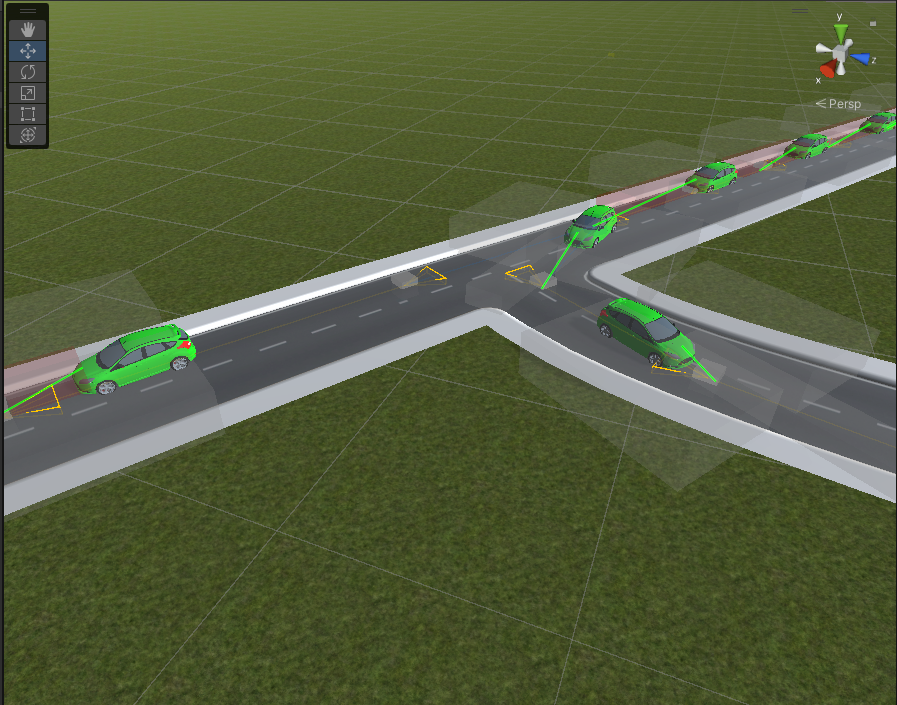
\includegraphics[width=.8\textwidth]{simple-traffic-system.png} 
    \caption{Simple Traffic System - A showcase of vehicles following a route}
    \label{fig-sts}
\end{figure}

\subsubsection{IVIS implementation}

This section will cover the implementation of the chosen C-ITS solution using the proposed 
MAS framework. Based on the specification, two agents will be created. The agents will be 
created by inheriting classes from the MAS framework components and implementing custom behavior, as 
well as using its pre-defined C-ITS communication modules to simulate V2X communication. 

\textbf{Connected Traffic Light} \smallskip \\
The Connected Traffic Light agent is the first actor in the Smart Routing implementation.
There will be only one instance of this agent in the simulation which will manage a 
single traffic light. This agent will monitor the number of vehicles in the queue at a
designated intersection and process the data to evaluate if congestion is forming. It informs
about its local traffic state via localized (meaning that message includes the traffic light's
location) DENM messages broadcasted to all connected road users.

Since the agent's behavior is constant, apart from broadcasted DENM message content (value of
Sub-Cause Code), the agent has got only one task, consisting of two Skills - 
\texttt{ITSCommunicationSkill} for messaging service and \texttt{MonitorQueueSkill} which 
changes broadcasted Sub-Cause Code based on discovered number of vehicles in the queue. 
For reference, the agent's composition can be seen in fig. (\ref{cd-trafficLight}) and 
the agent's activity diagram can be seen in fig. (\ref{ad-trafficLight}).


\begin{figure}[htbp]
    \centering
    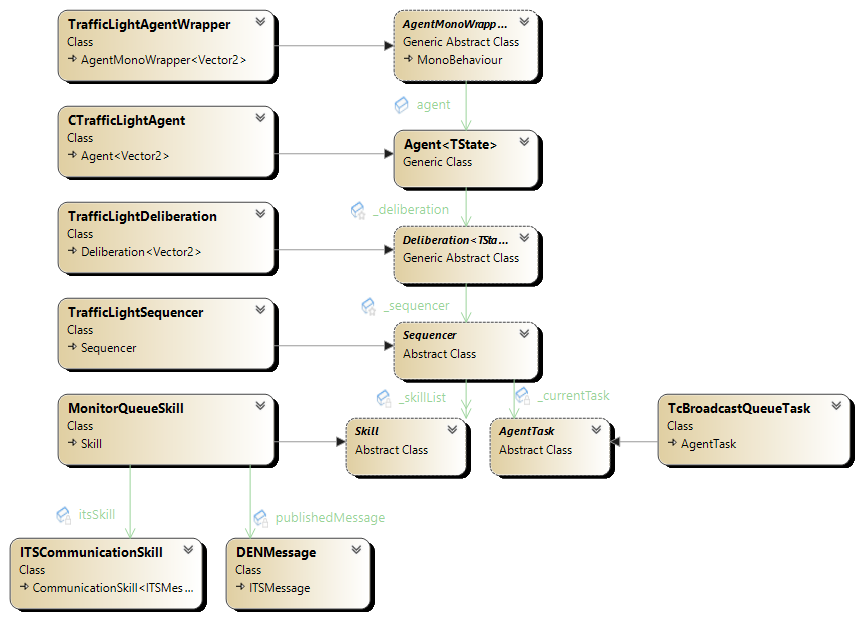
\includegraphics[width=.9\textwidth]{cd-SmartTrafficLight.png}
    \caption{Class diagram of the Connected Traffic Light implementation}
    \label{cd-trafficLight}
\end{figure}

\begin{figure}[htbp]
    \centering
    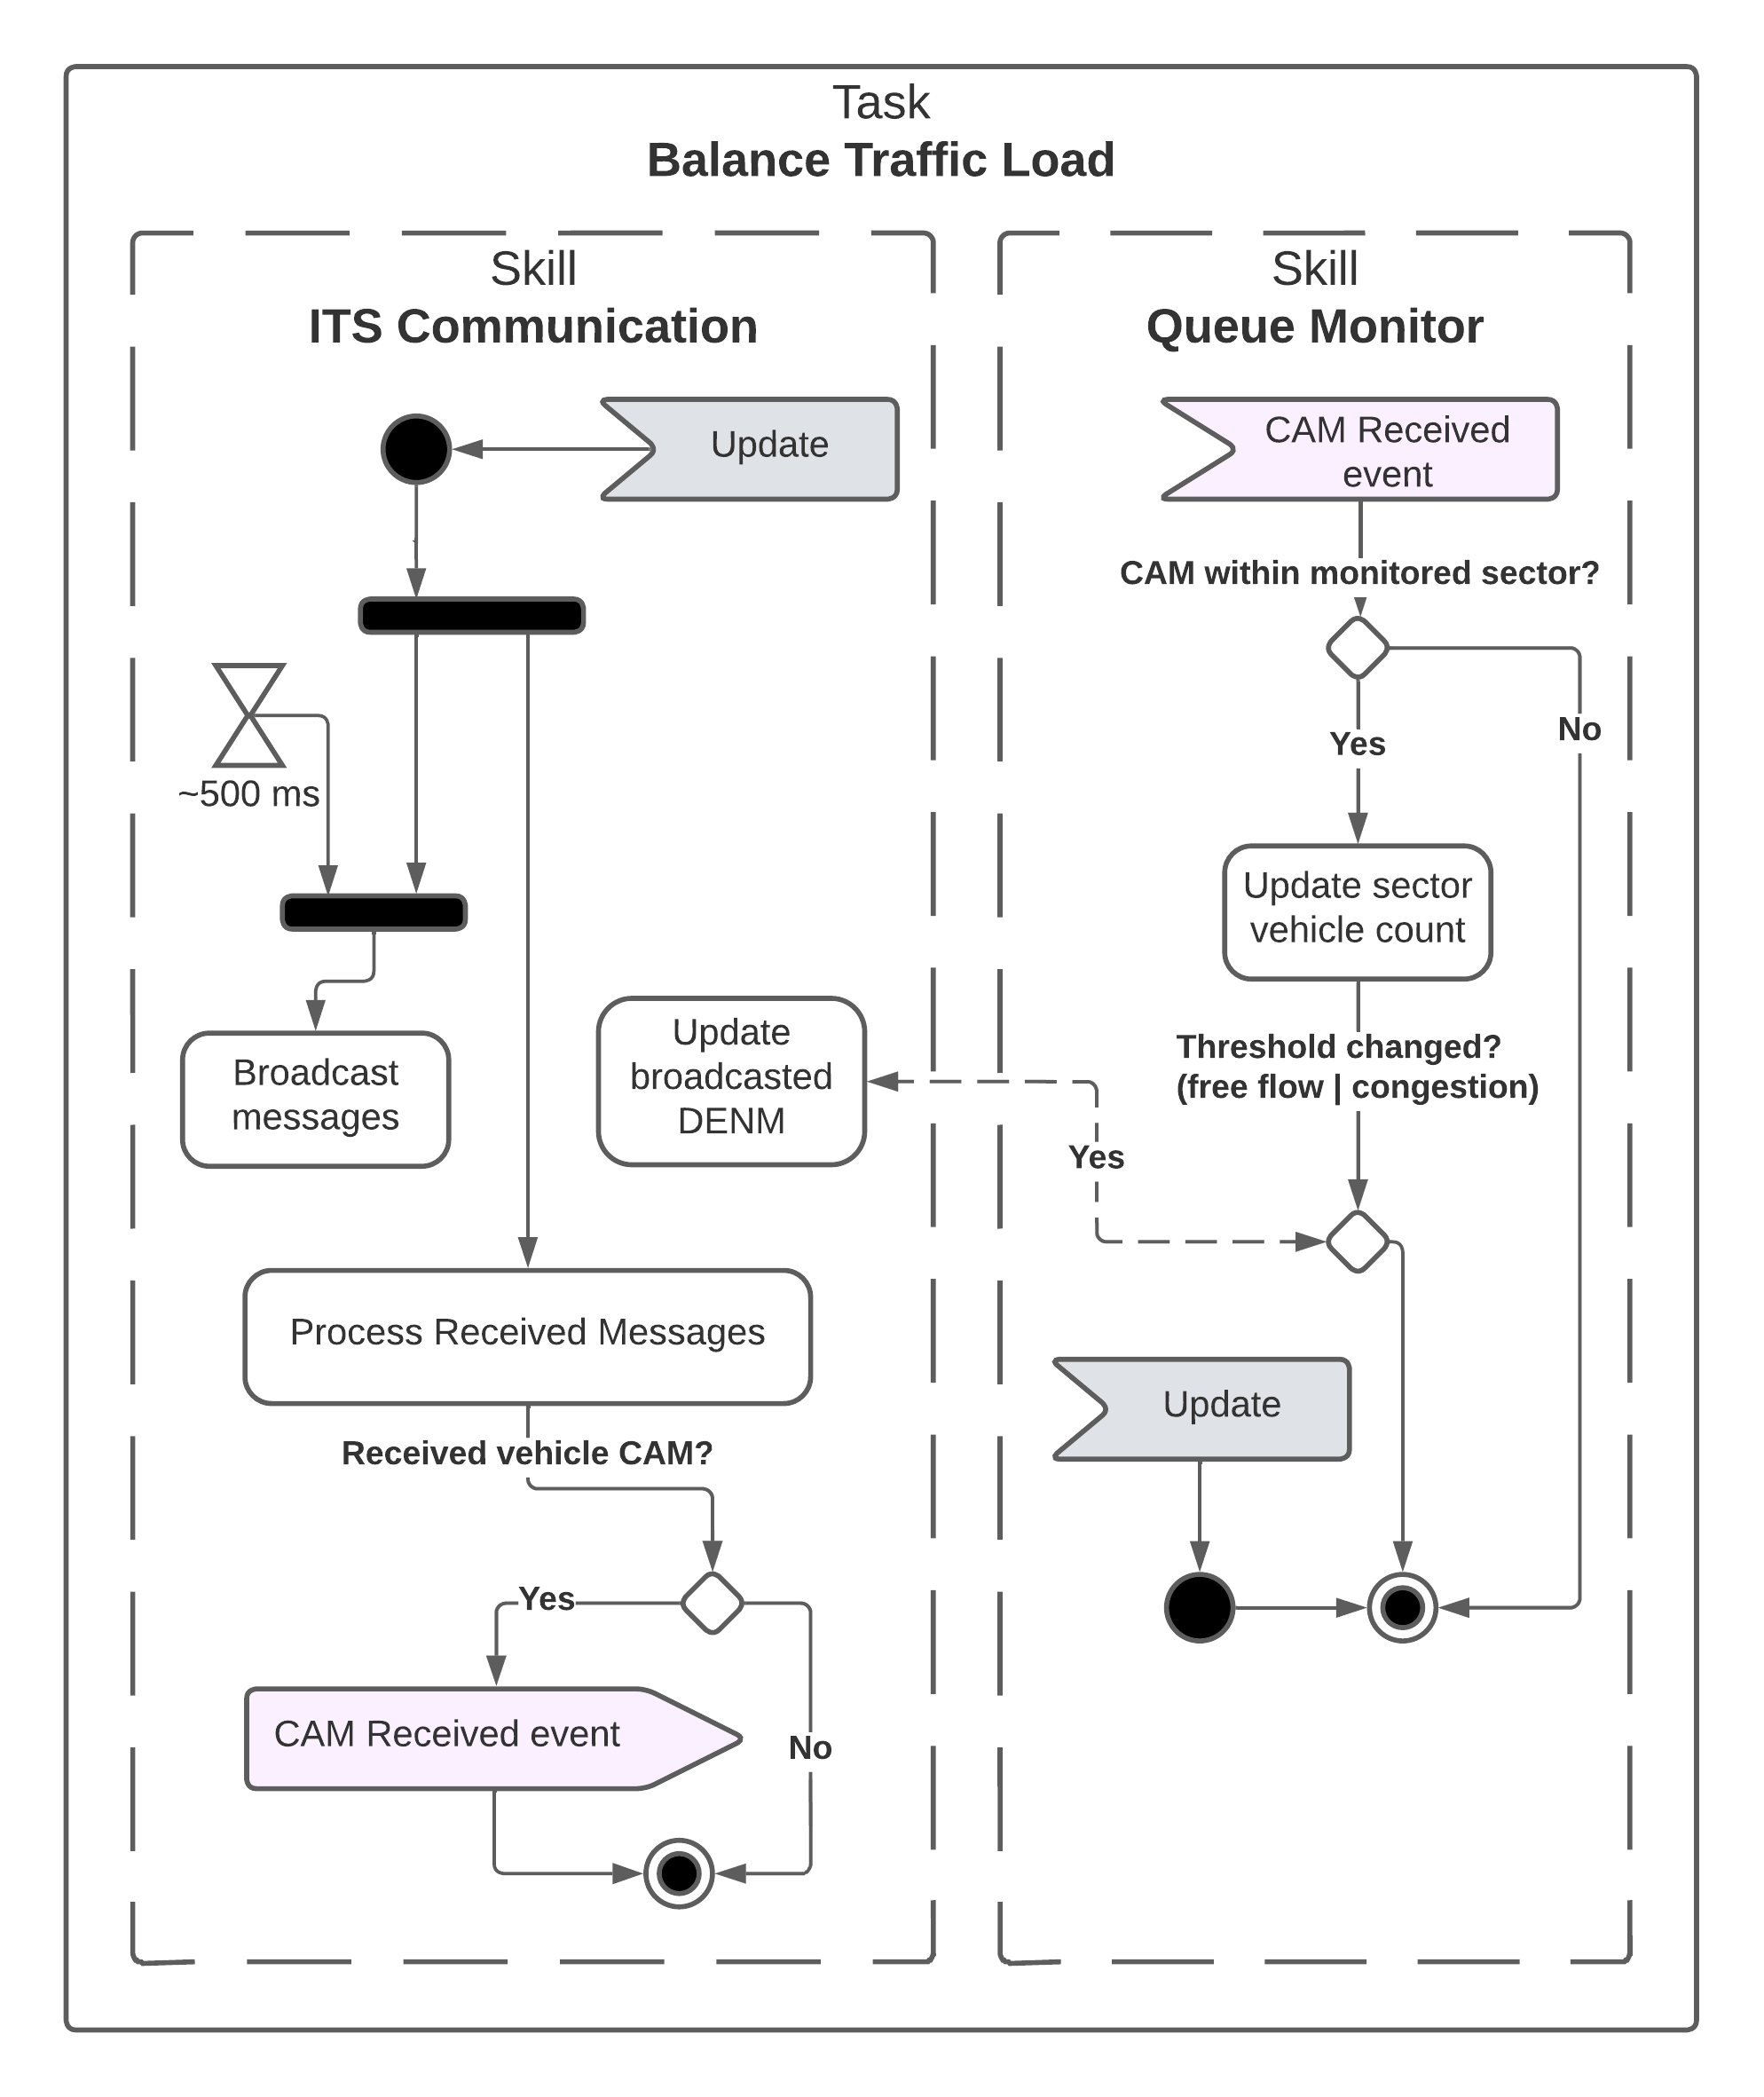
\includegraphics[width=.8\textwidth]{SmartTrafficLight.png}
    \caption{Activity diagram of the Connected Traffic Light agent}
    \label{ad-trafficLight}
\end{figure}

\textbf{Connected Vehicle} \smallskip \\
The Connected Vehicle agent is the second agent type in the simulation. This agent type is 
added as a component of each vehicle spawned in the simulation run. The purpose of this 
agent module is to process received DENM messages and evaluate if the planned route needs 
to be changed. It also broadcasts CAM messages to other road users. The content of 
broadcasted CAM messages is the vehicle's location.

Although there is only a single task defined in this agent, its initialization is 
parametrized, allowing the agent to adapt to the current conditions. The task consists of 
four Skills:

\begin{itemize}
    \item \texttt{ITSCommunicationSkill} - C-ITS messaging interface, as has been described before.
    \item \texttt{VehicleInfoSkill} - A Skill for retrieving information about the vehicle, namely 
    its current position, and additional navigation properties, which will be discussed separately.
    \item \texttt{CAMPositionUpdateSkill} - As the name suggests, this is a trivial "plumbing" Skill 
    that takes vehicle position from the foregoing Skill and updates the broadcasted CAM message of 
    the message service Skill accordingly.
    \item \texttt{CongestionMonitorSkill} - This Skill takes input from \texttt{VehicleInfoSkill} and 
    processes received DENM messages if there are updates about traffic conditions on the network. 
    Initially, it checks whether the DENM event location is along the planned route and throws the 
    message away if not. If there is congestion on the planned route, the Skill will find out and 
    trigger a Skill Interrupted event, which will signal to the Deliberation layer to re-plan the route. 
    Here, the parametrized initialization of the agent's task is utilized by providing a flag/switch to 
    plan the default or an alternative route. 
\end{itemize}

The agent's class diagram can be seen in figure (\ref{cd-smartRoutingVehicle}) and its activity diagram 
on figure (\ref{ad-smartRoutingVehicle}).

\begin{figure}[htbp]
    \centering
    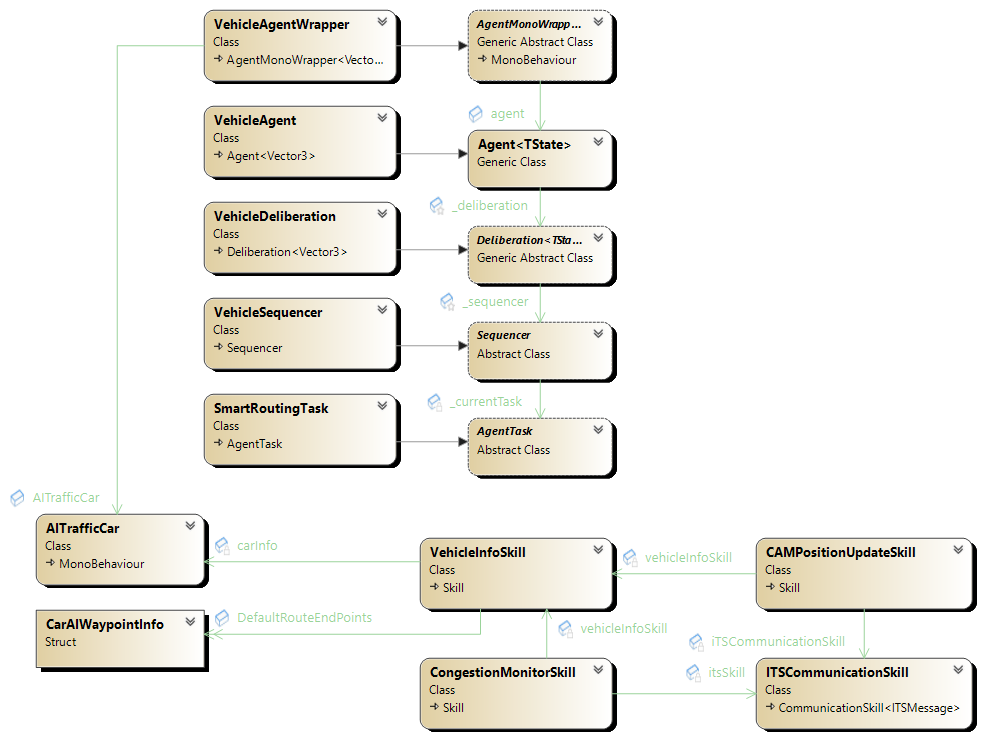
\includegraphics[width=.9\textwidth]{cd-SmartRoutingAgent.png}
    \caption{Class diagram of the Connected Vehicle implementation}
    \label{cd-smartRoutingVehicle}
\end{figure}

\begin{figure}[htbp]
    \centering
    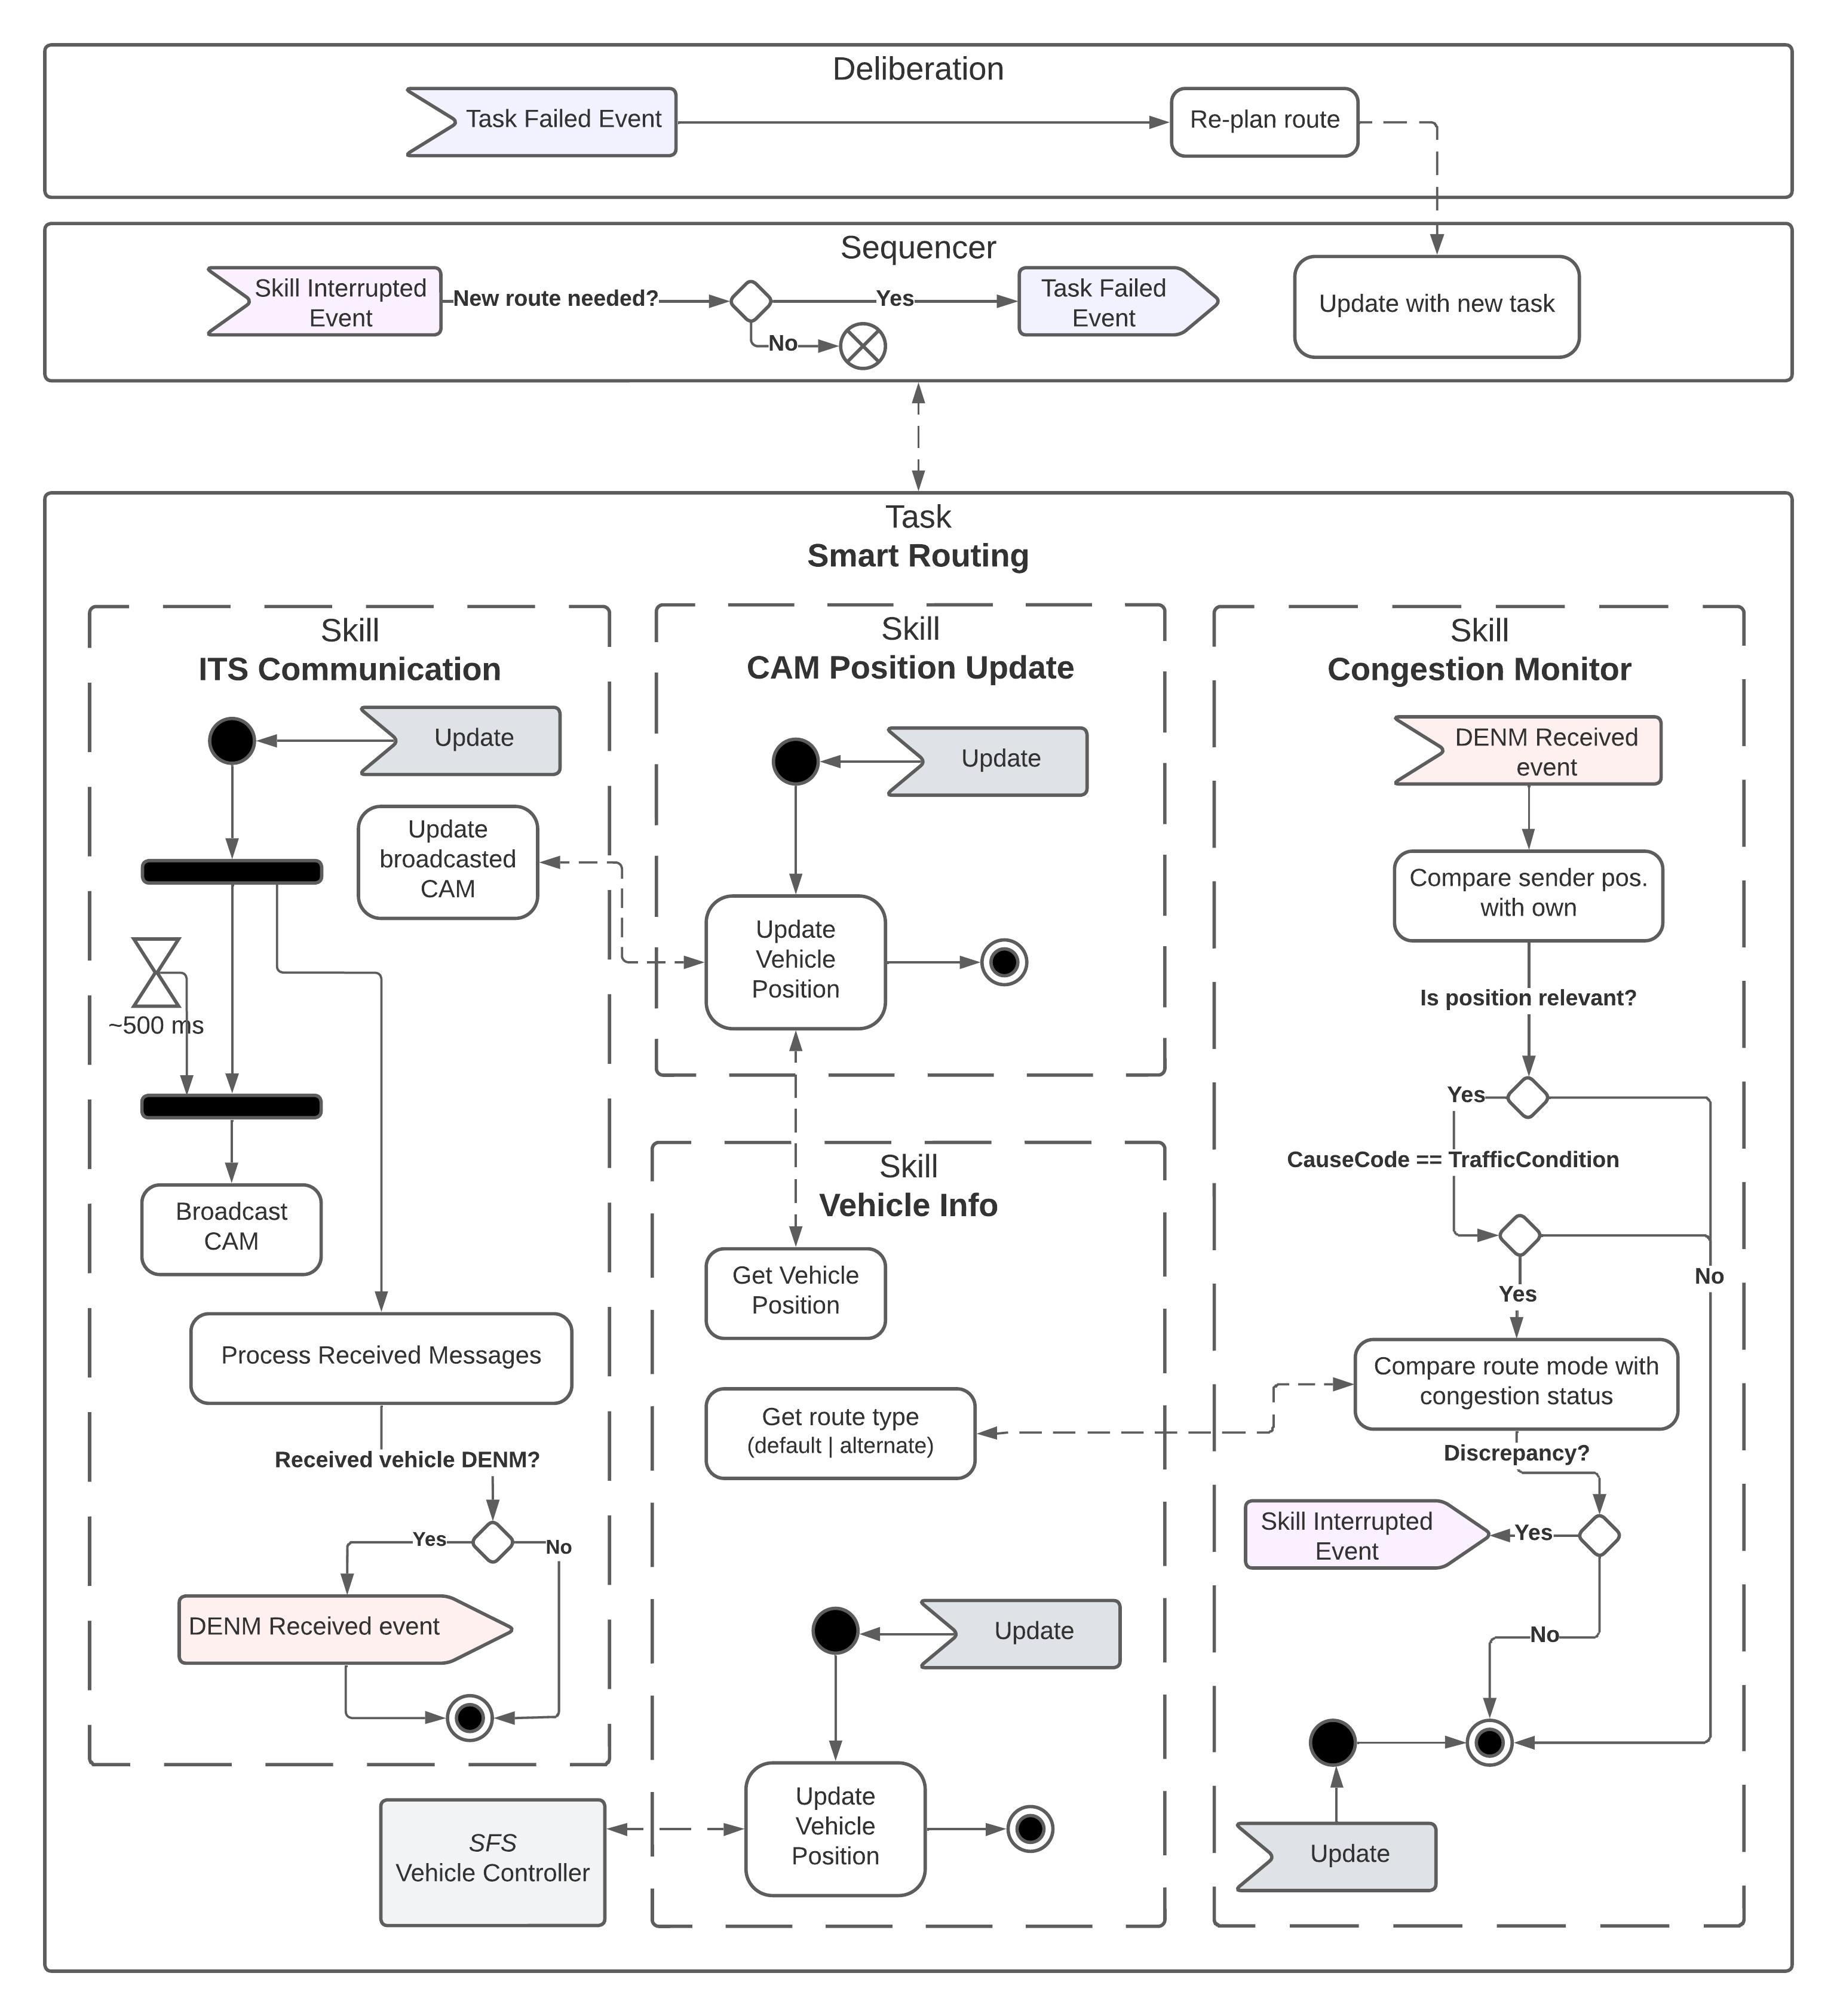
\includegraphics[width=.99\textwidth]{SmartRoutingVehicle.png}
    \caption{Activity diagram of the Connected Vehicle agent}
    \label{ad-smartRoutingVehicle}
\end{figure}

\textbf{Other modifications} \smallskip \newline
Since the information about vehicle navigation and route information is managed by the
\emph{Simple Traffic System} (STS) package scripts, modifications needed to be added to the
vehicle management and route management scripts. This mainly involved exposing private fields
to be publicly accessed or adding other ways how to modify inner properties from the outside,
so that the external MAS framework scripts can interact with them. The
\texttt{VehicleInfoSkill} provided an interface to manipulate required properties.
Additionally, the route-switching algorithm has been modified. In the original (STS) code,
a vehicle chooses a turn at an intersection randomly. The performed modifications allow outside 
code to decide which turn shall the vehicle take.

Regarding the simulation evaluation, a logging script has been created that can be used on the 
vehicles in the simulation logging object uptime and writing it into a log file. As a result, 
the time taken by each vehicle to reach its destination can be measured and further analyzed.

\subsubsection{Simulation set-up}

After describing the IVIS system implementation details, the simulation set-up and evaluation 
methodology will be described. 

Using the third-party packages, a road stretch has been created to test the implementation.
The road stretch features a primary route that has got a traffic light along the way, imitating 
an intersection. This route represents the shortest path route through an urban area. 
There is also a second route, which is considerably longer and winding, representing a countryside 
road with less average traffic intensity. A "warm-up" section where vehicles are spawned is
preceding the branch-off into the two routes. For visual reference, see Figure
(\ref{fig-routeMap}) below.

\begin{figure}[htbp]
    \centering
    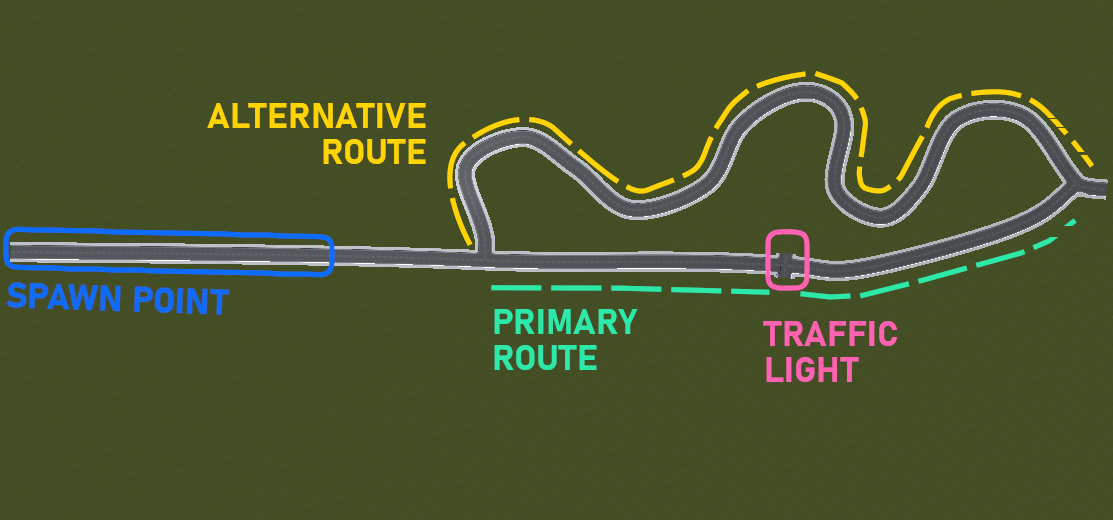
\includegraphics[width=.9\textwidth]{test-route-map-legend.png}
    \caption{Road stretch for simulating the IVIS system}
    \label{fig-routeMap}
\end{figure}

To verify and prove that the Smart Routing IVIS system works, simulations were run iteratively with 
parametrized traffic light queue size threshold for identifying congestion. The number 
of vehicles to drive through the road stretch was chosen to be $N_v = 20 $ and the queue size 
threshold ranged from $0..N_v$. To gather more results 
and avoid the risk of unknowingly analyzing an edge case parameter combination, the simulation batch 
was run multiple times with modified traffic flow influencing parameters. The variable parameters are:

\begin{itemize}
    \itemspacing{.7}
    \item Alternative route speed limit ($V_{alt}$)
    \item Green phase length ($T_{green}$)
    \item Yellow phase length ($T_{yellow}$)
\end{itemize}

The Table (\ref{tab-sims}) shows the three variations of chosen simulation parameters.

\begin{table}[htbp]
    \caption{Parameter values for simulation batches}
    \centering\begin{tabular}{lccc}
        \toprule
        \# & $V_{alt}$ & $T_{green}$ & $T_{yellow}$ \\ 
         & $[kmh^{-1}]$ & $[s]$ & $[s]$ \\ \midrule
        1 & 25  & 6 & 1 \\
        2 & 25  & 7 & 2 \\
        3 & 30  & 7 & 1 \\ \bottomrule
    \end{tabular}
    \label{tab-sims}
\end{table}

\subsubsection{Simulation results}

The simulations were successfully run and the logs containing travel time for each vehicle were processed 
and evaluated. The observed variables were \emph{Total travel time}, \emph{Maximum travel time}
and \emph{Minimum travel time}. The plotted simulation results are in Figures (\ref{fig-sim-ttt}) \& (\ref{fig-sim-minmax}).
Note that the plot legend conveys information about simulation parameters in format [ $V_{alt}$ - $T_{green}$ - $T_{yellow}$ ].

\begin{figure}[htbp]
    \centering
    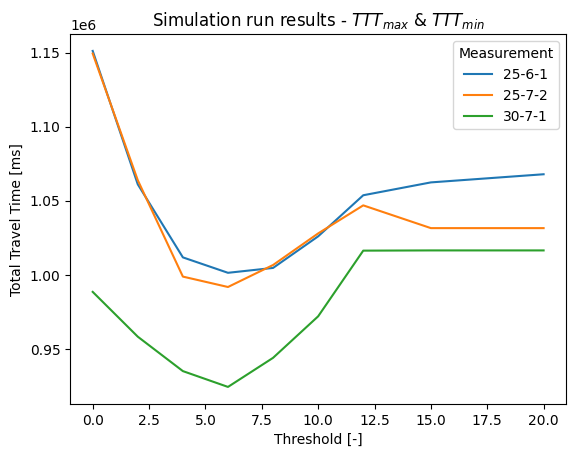
\includegraphics[width=.8\textwidth]{ttt.png}
    \caption{Simulation results - Total travel time}
    \label{fig-sim-ttt}
\end{figure}

\begin{figure}[htbp]
    \centering
    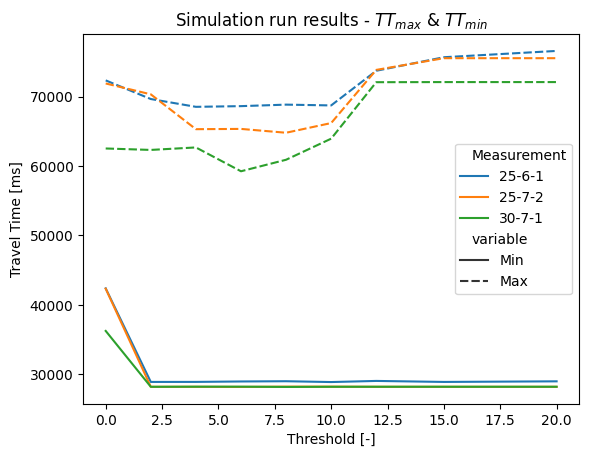
\includegraphics[width=.8\textwidth]{MinMax.png}
    \caption{Simulation results - Min and Max travel time}
    \label{fig-sim-minmax}
\end{figure}

When evaluating the simulation results, it is clear that the threshold value does influence the
travel time of vehicles, which is expected if the IVIS implementation is assumed to work. With
the threshold equal to zero, all vehicles take the alternative longer path and experience large
travel times. When the threshold gradually increases, allowing groups of vehicles onto the 
main route, the travel time starts decreasing rapidly, as the main route has enough capacity to clear 
the oncoming traffic without disruption. Around the threshold level of \textbf{six}, the traffic flow 
rate reaches the route's capacity and with increasing queue threshold the travel times start to
increase while rendering the alternative route under-utilized.

All three simulation batches do affect travel time (which implies that traffic flow 
is also affected) as expected. The absolute values of travel time have changed, however, 
the relative changes depending on queue threshold size were very similar in all three 
variations.

\clearpage 

\subsection{Conclusion}

In this chapter, an ITS solution for the framework validation has been chosen to implement
using the proposed framework, based on a qualitative analysis considering criteria determined
from preceding discussion and research. The system to implement was the Smart Routing C-ITS
utilizing V2I communication, dynamically re-planning optimal route to the destination. Requirements
for system implementation were defined to better evaluate the implementation results.
Afterward, third-party packages that facilitate validation scenario development were briefly
introduced, leading to agent type specification and their components, as well as
action diagrams outlining their behavior, while also addressing the required IVS package code
changes to ensure successful integration with the agent framework. Simulation methodology was
introduced and simulations were successfully run, after which the results were analyzed. From the 
simulation results, it was identified that the chosen system behaved as one would expect and it
was concluded that the implementation of the C-ITS system was successful. 


\end{document}